

\documentclass[11pt,fleqn]{book} % Default font size and left-justified equations

%%%%%%%%%%%%%%%%%%%%%%%%%%%%%%%%%%%%%%%%%
% The Legrand Orange Book
% Structural Definitions File
% Version 2.0 (9/2/15)
%
% Original author:
% Mathias Legrand (legrand.mathias@gmail.com) with modifications by:
% Vel (vel@latextemplates.com)
% 
% This file has been downloaded from:
% http://www.LaTeXTemplates.com
%
% License:
% CC BY-NC-SA 3.0 (http://creativecommons.org/licenses/by-nc-sa/3.0/)
%
%%%%%%%%%%%%%%%%%%%%%%%%%%%%%%%%%%%%%%%%%

%----------------------------------------------------------------------------------------
%	VARIOUS REQUIRED PACKAGES AND CONFIGURATIONS
%----------------------------------------------------------------------------------------

\usepackage[top=3cm,bottom=3cm,left=5.5cm,right=3cm,headsep=10pt,letterpaper,asymmetric]{geometry} % Page margins
% Could use 6cm margin on left 

\usepackage{graphicx} % Required for including pictures
\graphicspath{{Pictures/}} % Specifies the directory where pictures are stored

\usepackage{lipsum} % Inserts dummy text

\usepackage{tikz} % Required for drawing custom shapes

\usepackage[english]{babel} % English language/hyphenation

\usepackage{enumitem} % Customize lists
\setlist{noitemsep} % Reduce spacing between bullet points and numbered lists

\usepackage{booktabs} % Required for nicer horizontal rules in tables

\usepackage{xcolor} % Required for specifying colors by name
%\definecolor{rust}{RGB}{243,102,25} % Define the orange color used for highlighting throughout the book
\definecolor{rust}{RGB}{153, 0, 0} % Define alternate red color

\usepackage{pdftexcmds}



%----------------------------------------------------------------------------------------
%	FONTS
%----------------------------------------------------------------------------------------

\usepackage{avant} % Use the Avantgarde font for headings
%\usepackage{times} % Use the Times font for headings
\usepackage{mathptmx} % Use the Adobe Times Roman as the default text font together with math symbols from the Sym­bol, Chancery and Com­puter Modern fonts

\usepackage{microtype} % Slightly tweak font spacing for aesthetics
\usepackage[utf8]{inputenc} % Required for including letters with accents
\usepackage[T1]{fontenc} % Use 8-bit encoding that has 256 glyphs
\usepackage{relsize} % Allow relative font sizing
\renewcommand\RSlargest{100pt} 
%----------------------------------------------------------------------------------------
%	BIBLIOGRAPHY AND INDEX
%----------------------------------------------------------------------------------------

\usepackage[style=alphabetic,citestyle=numeric,sorting=nyt,sortcites=true,autopunct=true,babel=hyphen,hyperref=true,abbreviate=false,backref=true,backend=biber]{biblatex}
\addbibresource{bibliography.bib} % BibTeX bibliography file
\defbibheading{bibempty}{}

\usepackage{calc} % For simpler calculation - used for spacing the index letter headings correctly
\usepackage{makeidx} % Required to make an index
\makeindex % Tells LaTeX to create the files required for indexing

%----------------------------------------------------------------------------------------
%	MAIN TABLE OF CONTENTS
%----------------------------------------------------------------------------------------

\usepackage{titletoc} % Required for manipulating the table of contents

\contentsmargin{0cm} % Removes the default margin

% Part text styling
\titlecontents{part}[0cm]
{\addvspace{20pt}\centering\large\bfseries}
{}
{}
{}

% Chapter text styling
\titlecontents{chapter}[1.25cm] % Indentation
{\addvspace{12pt}\large\sffamily\bfseries} % Spacing and font options for chapters
{\color{rust!60}\contentslabel[\Large\thecontentslabel]{1.25cm}\color{rust}} % Chapter number
{\color{rust}}  
{\color{rust!60}\normalsize\;\titlerule*[.5pc]{.}\;\thecontentspage} % Page number

% Section text styling
\titlecontents{section}[1.25cm] % Indentation
{\addvspace{3pt}\sffamily\bfseries} % Spacing and font options for sections
{\contentslabel[\thecontentslabel]{1.25cm}} % Section number
{}
{\hfill\color{black}\thecontentspage} % Page number
[]

% Subsection text styling
\titlecontents{subsection}[1.25cm] % Indentation
{\addvspace{1pt}\sffamily\small} % Spacing and font options for subsections
{\contentslabel[\thecontentslabel]{1.25cm}} % Subsection number
{}
{\ \titlerule*[.5pc]{.}\;\thecontentspage} % Page number
[]

% List of figures
\titlecontents{figure}[0em]
{\addvspace{-5pt}\sffamily}
{\thecontentslabel\hspace*{1em}}
{}
{\ \titlerule*[.5pc]{.}\;\thecontentspage}
[]

% List of tables
\titlecontents{table}[0em]
{\addvspace{-5pt}\sffamily}
{\thecontentslabel\hspace*{1em}}
{}
{\ \titlerule*[.5pc]{.}\;\thecontentspage}
[]

%----------------------------------------------------------------------------------------
%	MINI TABLE OF CONTENTS IN PART HEADS
%----------------------------------------------------------------------------------------

% Chapter text styling
\titlecontents{lchapter}[0em] % Indenting
{\addvspace{15pt}\large\sffamily\bfseries} % Spacing and font options for chapters
{\color{rust}\contentslabel[\Large\thecontentslabel]{1.25cm}\color{rust}} % Chapter number
{}  
{\color{rust}\normalsize\sffamily\bfseries\;\titlerule*[.5pc]{.}\;\thecontentspage} % Page number

% Section text styling
\titlecontents{lsection}[0em] % Indenting
{\sffamily\small} % Spacing and font options for sections
{\contentslabel[\thecontentslabel]{1.25cm}} % Section number
{}
{}

% Subsection text styling
\titlecontents{lsubsection}[.5em] % Indentation
{\normalfont\footnotesize\sffamily} % Font settings
{}
{}
{}

%----------------------------------------------------------------------------------------
%	PAGE HEADERS
%----------------------------------------------------------------------------------------

\usepackage{fancyhdr} % Required for header and footer configuration

\pagestyle{fancy}
\renewcommand{\chaptermark}[1]{\markboth{\sffamily\normalsize\bfseries\chaptername\ \thechapter.\ #1}{}} % Chapter text font settings
\renewcommand{\sectionmark}[1]{\markright{\sffamily\normalsize\thesection\hspace{5pt}#1}{}} % Section text font settings
\fancyhf{} \fancyhead[LE,RO]{\sffamily\normalsize\thepage} % Font setting for the page number in the header
\fancyhead[LO]{\rightmark} % Print the nearest section name on the left side of odd pages
\fancyhead[RE]{\leftmark} % Print the current chapter name on the right side of even pages
\renewcommand{\headrulewidth}{0.5pt} % Width of the rule under the header
\addtolength{\headheight}{2.5pt} % Increase the spacing around the header slightly
\renewcommand{\footrulewidth}{0pt} % Removes the rule in the footer
\fancypagestyle{plain}{\fancyhead{}\renewcommand{\headrulewidth}{0pt}} % Style for when a plain pagestyle is specified

% Removes the header from odd empty pages at the end of chapters
\makeatletter
\renewcommand{\cleardoublepage}{
\clearpage\ifodd\c@page\else
\hbox{}
\vspace*{\fill}
\thispagestyle{empty}
\newpage
\fi}

%----------------------------------------------------------------------------------------
%	THEOREM STYLES
%----------------------------------------------------------------------------------------

\usepackage{amsmath,amsfonts,amssymb,amsthm} % For math equations, theorems, symbols, etc

\newcommand{\intoo}[2]{\mathopen{]}#1\,;#2\mathclose{[}}
\newcommand{\ud}{\mathop{\mathrm{{}d}}\mathopen{}}
\newcommand{\intff}[2]{\mathopen{[}#1\,;#2\mathclose{]}}
\newtheorem{notation}{Notation}[chapter]

% Boxed/framed environments
\newtheoremstyle{rustnumbox}% % Theorem style name
{0pt}% Space above
{0pt}% Space below
{\normalfont}% % Body font
{}% Indent amount
{\small\bf\sffamily\color{rust}}% % Theorem head font
{\;}% Punctuation after theorem head
{0.25em}% Space after theorem head
{\small\sffamily\color{rust}\thmname{#1}\nobreakspace\thmnumber{\@ifnotempty{#1}{}\@upn{#2}}% Theorem text (e.g. Theorem 2.1)
\thmnote{\nobreakspace\the\thm@notefont\sffamily\bfseries\color{black}---\nobreakspace#3.}} % Optional theorem note
\renewcommand{\qedsymbol}{$\blacksquare$}% Optional qed square

\newtheoremstyle{blacknumex}% Theorem style name
{5pt}% Space above
{5pt}% Space below
{\normalfont}% Body font
{} % Indent amount
{\small\bf\sffamily}% Theorem head font
{\;}% Punctuation after theorem head
{0.25em}% Space after theorem head
{\small\sffamily{\tiny\ensuremath{\blacksquare}}\nobreakspace\thmname{#1}\nobreakspace\thmnumber{\@ifnotempty{#1}{}\@upn{#2}}% Theorem text (e.g. Theorem 2.1)
\thmnote{\nobreakspace\the\thm@notefont\sffamily\bfseries---\nobreakspace#3.}}% Optional theorem note

\newtheoremstyle{blacknumbox} % Theorem style name
{0pt}% Space above
{0pt}% Space below
{\normalfont}% Body font
{}% Indent amount
{\small\bf\sffamily}% Theorem head font
{\;}% Punctuation after theorem head
{0.25em}% Space after theorem head
{\small\sffamily\thmname{#1}\nobreakspace\thmnumber{\@ifnotempty{#1}{}\@upn{#2}}% Theorem text (e.g. Theorem 2.1)
\thmnote{\nobreakspace\the\thm@notefont\sffamily\bfseries---\nobreakspace#3.}}% Optional theorem note

% Non-boxed/non-framed environments
\newtheoremstyle{rustnum}% % Theorem style name
{5pt}% Space above
{5pt}% Space below
{\normalfont}% % Body font
{}% Indent amount
{\small\bf\sffamily\color{rust}}% % Theorem head font
{\;}% Punctuation after theorem head
{0.25em}% Space after theorem head
{\small\sffamily\color{rust}\thmname{#1}\nobreakspace\thmnumber{\@ifnotempty{#1}{}\@upn{#2}}% Theorem text (e.g. Theorem 2.1)
\thmnote{\nobreakspace\the\thm@notefont\sffamily\bfseries\color{black}---\nobreakspace#3.}} % Optional theorem note
\renewcommand{\qedsymbol}{$\blacksquare$}% Optional qed square
\makeatother

% Defines the theorem text style for each type of theorem to one of the three styles above
\newcounter{dummy} 
\numberwithin{dummy}{section}
\theoremstyle{rustnumbox}
\newtheorem{theoremeT}[dummy]{Theorem}
\newtheorem{assignment}{Assignment}[chapter]

\newtheorem{exerciseT}{Exercise}[chapter]
\theoremstyle{blacknumex}
\newtheorem{exampleT}{Example}[chapter]
\theoremstyle{blacknumbox}
\newtheorem{vocabulary}{Vocabulary}[chapter]
\newtheorem{definitionT}{Definition}[section]
\newtheorem{corollaryT}[dummy]{Corollary}
\theoremstyle{rustnum}
\newtheorem{proposition}[dummy]{Proposition}

%----------------------------------------------------------------------------------------
%	DEFINITION OF COLORED BOXES
%----------------------------------------------------------------------------------------

\RequirePackage[framemethod=default]{mdframed} % Required for creating the theorem, definition, exercise and corollary boxes

% Theorem box
\newmdenv[skipabove=7pt,
skipbelow=7pt,
backgroundcolor=black!5,
linecolor=rust,
innerleftmargin=5pt,
innerrightmargin=5pt,
innertopmargin=5pt,
leftmargin=0cm,
rightmargin=0cm,
innerbottommargin=5pt]{tBox}

% Exercise box	  
\newmdenv[skipabove=7pt,
skipbelow=7pt,
rightline=false,
leftline=true,
topline=false,
bottomline=false,
backgroundcolor=rust!10,
linecolor=rust,
innerleftmargin=5pt,
innerrightmargin=5pt,
innertopmargin=5pt,
innerbottommargin=5pt,
leftmargin=0cm,
rightmargin=0cm,
linewidth=4pt]{eBox}	

% Definition box
\newmdenv[skipabove=7pt,
skipbelow=7pt,
rightline=false,
leftline=true,
topline=false,
bottomline=false,
linecolor=rust,
innerleftmargin=5pt,
innerrightmargin=5pt,
innertopmargin=0pt,
leftmargin=0cm,
rightmargin=0cm,
linewidth=4pt,
innerbottommargin=0pt]{dBox}	

% Corollary box
\newmdenv[skipabove=7pt,
skipbelow=7pt,
rightline=false,
leftline=true,
topline=false,
bottomline=false,
linecolor=gray,
backgroundcolor=black!5,
innerleftmargin=5pt,
innerrightmargin=5pt,
innertopmargin=5pt,
leftmargin=0cm,
rightmargin=0cm,
linewidth=4pt,
innerbottommargin=5pt]{cBox}

% Creates an environment for each type of theorem and assigns it a theorem text style from the "Theorem Styles" section above and a colored box from above
\newenvironment{theorem}{\begin{tBox}\begin{theoremeT}}{\end{theoremeT}\end{tBox}}
\newenvironment{exercise}{\begin{eBox}\begin{exerciseT}}{\hfill{\color{rust}\tiny\ensuremath{\blacksquare}}\end{exerciseT}\end{eBox}}				  
\newenvironment{definition}{\begin{dBox}\begin{definitionT}}{\end{definitionT}\end{dBox}}	
\newenvironment{example}{\begin{exampleT}}{\hfill{\tiny\ensuremath{\blacksquare}}\end{exampleT}}		
\newenvironment{corollary}{\begin{cBox}\begin{corollaryT}}{\end{corollaryT}\end{cBox}}	

%----------------------------------------------------------------------------------------
%	WARNING ENVIRONMENT
%----------------------------------------------------------------------------------------

\newenvironment{warning}{\par\vspace{10pt}\small % Vertical white space above the remark and smaller font size
	\begin{list}{}{
			\leftmargin=35pt % Indentation on the left
			\rightmargin=25pt}\item\ignorespaces % Indentation on the right
		\makebox[-2.5pt]{\begin{tikzpicture}[overlay]
			\node[draw=rust!60,line width=1pt,circle,fill=rust!25,font=\sffamily\bfseries,inner sep=2pt,outer sep=0pt] at (-15pt,0pt){\textcolor{rust}{\textbf{!}}};\end{tikzpicture}} 
		\advance\baselineskip -1pt}{\end{list}\vskip5pt} % Tighter line spacing and white space after remark

%----------------------------------------------------------------------------------------
%	REMARK ENVIRONMENT
%----------------------------------------------------------------------------------------

\newenvironment{remark}{\par\vspace{10pt}\small % Vertical white space above the remark and smaller font size
\begin{list}{}{
\leftmargin=35pt % Indentation on the left
\rightmargin=25pt}\item\ignorespaces % Indentation on the right
\makebox[-2.5pt]{\begin{tikzpicture}[overlay]
\node[draw=rust!60,line width=1pt,circle,fill=rust!25,font=\sffamily\bfseries,inner sep=2pt,outer sep=0pt] at (-15pt,0pt){\textcolor{rust}{R}};\end{tikzpicture}} % Orange R in a circle
\advance\baselineskip -1pt}{\end{list}\vskip5pt} % Tighter line spacing and white space after remark

%----------------------------------------------------------------------------------------
%	SECTION NUMBERING IN THE MARGIN
%----------------------------------------------------------------------------------------

\makeatletter

% just bottom line
%\newmdenv[topline=false,leftline=false,rightline=false]{test123}

%\newmdenv[
%rightline=false, leftline=false, topline=false, bottomline=true,
%linecolor=rust, linewidth=4pt
%]{sectionUnderline}

% Adjusts all numbering for sections and subsections
\renewcommand{\@seccntformat}[1]{  
    \ifnum\pdf@strcmp{#1}{section}=\z@ 
    
    %\llap{\colorbox{gray!15}{\makebox[3.25cm][r]{\textcolor{gray}{\textsc{\@nameuse{secTypeName}}\hspace{0.5em}\relsize{1.25}\textcolor{rust}{\csname the#1\endcsname}}}}\hspace{.5em}}
    \llap{
        %\begin{sectionUnderline}
            \makebox[3.25cm][r]{\textcolor{gray}{\textsc{\@nameuse{secTypeName}}\hspace{0.5em}\relsize{1.25}\textcolor{rust}{\csname the#1\endcsname}}}
            \textcolor{rust}{\hspace{-3.25cm}\rule[-.2cm]{3.13cm}{2pt}}
        %\end{sectionUnderline}
        \hspace{.5em}
    }
    \else
    \llap{\textcolor{rust}{\csname the#1\endcsname}\hspace{1em}}%
    \fi 
   % \llap{\textcolor{rust}{\csname the#1\endcsname}\hspace{1em}}
}  % hspace controls spacing of section number to section name    


\newcommand{\setSectionType}[1]{
    \@namedef{secTypeName}{#1}
}
        
\renewcommand{\section}{\@startsection{section}{1}{-8pt}
{-5ex \@plus -1ex \@minus -.2ex}
{2.0ex \@plus.2ex }
{\normalfont\large\sffamily\bfseries}}


\renewcommand{\subsection}{\@startsection {subsection}{2}{-3pt}
{-3ex \@plus -0.1ex \@minus -.4ex}
{0.5ex \@plus.2ex }
{\normalfont\sffamily\bfseries}}
\renewcommand{\subsubsection}{\@startsection {subsubsection}{3}{\z@}
{-2ex \@plus -0.1ex \@minus -.2ex}
{.2ex \@plus.2ex }
{\normalfont\small\sffamily\bfseries}}                        
\renewcommand\paragraph{\@startsection{paragraph}{4}{\z@}
{-2ex \@plus-.2ex \@minus .2ex}
{.1ex}
{\normalfont\small\sffamily\bfseries}}

%----------------------------------------------------------------------------------------
%	PART HEADINGS
%----------------------------------------------------------------------------------------

% numbered part in the table of contents
\newcommand{\@mypartnumtocformat}[2]{%
\setlength\fboxsep{0pt}%
\noindent\colorbox{rust!20}{\strut\parbox[c][.7cm]{\ecart}{\color{rust!70}\Large\sffamily\bfseries\centering#1}}\hskip\esp\colorbox{rust!40}{\strut\parbox[c][.7cm]{\linewidth-\ecart-\esp}{\Large\sffamily\centering#2}}}%
%%%%%%%%%%%%%%%%%%%%%%%%%%%%%%%%%%
% unnumbered part in the table of contents
\newcommand{\@myparttocformat}[1]{%
\setlength\fboxsep{0pt}%
\noindent\colorbox{rust!40}{\strut\parbox[c][.7cm]{\linewidth}{\Large\sffamily\centering#1}}}%
%%%%%%%%%%%%%%%%%%%%%%%%%%%%%%%%%%
\newlength\esp
\setlength\esp{4pt}
\newlength\ecart
\setlength\ecart{1.2cm-\esp}
\newcommand{\thepartimage}{}%
\newcommand{\partimage}[1]{\renewcommand{\thepartimage}{#1}}%
\def\@part[#1]#2{%
\ifnum \c@secnumdepth >-2\relax%
\refstepcounter{part}%
\addcontentsline{toc}{part}{\texorpdfstring{\protect\@mypartnumtocformat{\thepart}{#1}}{\partname~\thepart\ ---\ #1}}
\else%
\addcontentsline{toc}{part}{\texorpdfstring{\protect\@myparttocformat{#1}}{#1}}%
\fi%
\startcontents%
\markboth{}{}%
{\thispagestyle{empty}%
\begin{tikzpicture}[remember picture,overlay]%
\node at (current page.north west){\begin{tikzpicture}[remember picture,overlay]%	
\node[anchor=north] at (4cm,-3.25cm){\color{rust!60}\fontsize{220}{100}\sffamily\bfseries\@Roman\c@part}; 
\node[anchor=south east] at (\paperwidth-1cm,-\paperheight+1cm){\parbox[t][][t]{8.5cm}{
\printcontents{l}{0}{\setcounter{tocdepth}{1}}%
}};
\node[anchor=north east] at (\paperwidth-1.5cm,-3.25cm){\parbox[t][][t]{15cm}{\strut\raggedleft\color{black!40}\fontsize{30}{30}\sffamily\bfseries#2}};
\end{tikzpicture}};
\end{tikzpicture}}%
\@endpart}
\def\@spart#1{%
\startcontents%
\phantomsection
{\thispagestyle{empty}%
\begin{tikzpicture}[remember picture,overlay]%
\node at (current page.north west){\begin{tikzpicture}[remember picture,overlay]%	
\fill[rust!20](0cm,0cm) rectangle (\paperwidth,-\paperheight);
\node[anchor=north east] at (\paperwidth-1.5cm,-3.25cm){\parbox[t][][t]{15cm}{\strut\raggedleft\color{white}\fontsize{30}{30}\sffamily\bfseries#1}};
\end{tikzpicture}};
\end{tikzpicture}}
\addcontentsline{toc}{part}{\texorpdfstring{%
\setlength\fboxsep{0pt}%
\noindent\protect\colorbox{rust!40}{\strut\protect\parbox[c][.7cm]{\linewidth}{\Large\sffamily\protect\centering #1\quad\mbox{}}}}{#1}}%
\@endpart}
\def\@endpart{\vfil\newpage
\if@twoside
\if@openright
\null
\thispagestyle{empty}%
\newpage
\fi
\fi
\if@tempswa
\twocolumn
\fi}

%----------------------------------------------------------------------------------------
%	CHAPTER HEADINGS
%----------------------------------------------------------------------------------------

% A switch to conditionally include a picture, implemented by  Christian Hupfer
\newif\ifusechapterimage
\usechapterimagetrue
\newcommand{\thechapterimage}{}%
\newcommand{\chapterimage}[1]{\ifusechapterimage\renewcommand{\thechapterimage}{#1}\fi}%
\def\@makechapterhead#1{%
{\parindent \z@ \raggedright \normalfont
\ifnum \c@secnumdepth >\m@ne
\if@mainmatter
\begin{tikzpicture}[remember picture,overlay]
\node at (current page.north west)
{\begin{tikzpicture}[remember picture,overlay]
\node[anchor=north west,inner sep=0pt] at (0,0) {\ifusechapterimage\includegraphics[width=\paperwidth]{\thechapterimage}\fi};
%\draw[anchor=west] (\Gm@lmargin,-9cm) node [line width=2pt,rounded corners=15pt,draw=rust,fill=white,fill opacity=0.5,inner sep=15pt]{\strut\makebox[22cm]{}};

%%%%% Chapter text sizing
%\draw[anchor=west] (\Gm@lmargin-1.3cm,-4cm) node [line width=2pt,rounded corners=15pt,draw=rust,fill=white,fill opacity=0.75,inner sep=15pt]{\strut\makebox[22cm]{}};

%\draw[anchor=west] (\Gm@lmargin-1cm,-4.1cm) node {\huge\sffamily\bfseries\color{black}\thechapter. #1\strut};

% Use larger chapter number

\draw[anchor=west] (\Gm@lmargin-1.3cm,-3.9cm) node [line width=2pt,rounded corners=8pt,draw=rust,fill=white,fill opacity=0.75,inner sep=15pt]{\strut\makebox[22cm]{}};

\draw[anchor=west] (\Gm@lmargin-1cm,-4.0cm) node {\huge\sffamily\bfseries\color{black}{\relsize{2}\thechapter. }#1\strut};


\end{tikzpicture}};
\end{tikzpicture}
\else
\begin{tikzpicture}[remember picture,overlay]
\node at (current page.north west)
{\begin{tikzpicture}[remember picture,overlay]
\node[anchor=north west,inner sep=0pt] at (0,0) {\ifusechapterimage\includegraphics[width=\paperwidth]{\thechapterimage}\fi};
%\draw[anchor=west] (\Gm@lmargin,-9cm) node [line width=2pt,rounded corners=15pt,draw=rust,fill=white,fill opacity=0.5,inner sep=15pt]{\strut\makebox[22cm]{}};

\draw[anchor=west] (\Gm@lmargin,-4cm) node [line width=2pt,rounded corners=15pt,draw=rust,fill=white,fill opacity=0.75,inner sep=15pt]{\strut\makebox[22cm]{}};

\draw[anchor=west] (\Gm@lmargin+.3cm,-4cm) node {\huge\sffamily\bfseries\color{black}#1\strut};
\end{tikzpicture}};
\end{tikzpicture}
%\fi\fi\par\vspace*{270\p@}}}

\fi\fi\par\vspace*{150\p@}}}

%-------------------------------------------

\def\@makeschapterhead#1{%
\begin{tikzpicture}[remember picture,overlay]
\node at (current page.north west)
{\begin{tikzpicture}[remember picture,overlay]
\node[anchor=north west,inner sep=0pt] at (0,0) {\ifusechapterimage\includegraphics[width=\paperwidth]{\thechapterimage}\fi};
\draw[anchor=west] (\Gm@lmargin,-9cm) node [line width=2pt,rounded corners=15pt,draw=rust,fill=white,fill opacity=0.5,inner sep=15pt]{\strut\makebox[22cm]{}};
\draw[anchor=west] (\Gm@lmargin+.3cm,-9cm) node {\huge\sffamily\bfseries\color{black}#1\strut};
\end{tikzpicture}};
\end{tikzpicture}
\par\vspace*{270\p@}}
\makeatother

%----------------------------------------------------------------------------------------
%	HYPERLINKS IN THE DOCUMENTS
%----------------------------------------------------------------------------------------

\usepackage{hyperref}
\hypersetup{hidelinks,backref=true,pagebackref=true,hyperindex=true,colorlinks=false,breaklinks=true,urlcolor= rust,bookmarks=true,bookmarksopen=false,pdftitle={Lab Manual},pdfauthor={Brent Mellor}}
\usepackage{bookmark}
\bookmarksetup{
open,
numbered,
addtohook={%
\ifnum\bookmarkget{level}=0 % chapter
\bookmarksetup{bold}%
\fi
\ifnum\bookmarkget{level}=-1 % part
\bookmarksetup{color=rust,bold}%
\fi
}
}
 % Insert the commands.tex file which contains the majority of the structure behind the template
\usepackage{float}

\usepackage{listings} 
\lstset
{ 
    language=C,
    basicstyle=\ttfamily,
    columns=fullflexible,
    keepspaces=true,
    numbers=none,
    stepnumber=1,
    showstringspaces=false,
    tabsize=1,
    breaklines=true,
    breakatwhitespace=false,
    keywordstyle=\color{blue!80!black},
    stringstyle=\color{red!80!black},
    commentstyle=\color{green!40!black},
    morecomment=[l][\color{magenta!80!black}]{\#}
}

\usepackage{caption}
\captionsetup[figure]{font=small,skip=10pt}

%\usepackage{enumitem}
%\setlist{noitemsep} % or \setlist{noitemsep} to leave space around whole list


%%%%% May be too harsh to prevent paragraph breaks across pages! 
%\interlinepenalty 10000
\widowpenalties 1 10000
\raggedbottom


\newcommand{\ilcode}[1]{
    %\vspace{0.5pt}
    \smallskip
    \colorbox{gray!20!white}{
        \centering
        \parbox{\linewidth-2\fboxsep}{
            \lstinline@#1@
        }
    }
    %\vspace{0.5pt}
}

\newcommand{\code}[3]{
    \begin{figure}[]
        \colorbox{gray!20!white}{
            \parbox{\linewidth-2\fboxsep} {
                \centering 
                \lstinputlisting[language=C]{#1}
            }
        }
        \caption{#2}
        \label{#3}
    \end{figure}
}




\usepackage{textcomp}
\usepackage{wrapfig}
\usepackage{float}

\usepackage{silence} % http://ctan.org/pkg/silence
\ErrorFilter{textcomp}{Symbol \textrightarrow not provided}

% Disable paragraph indentation globally since template was indenting some and not others. (looked terrible)
\setlength{\parindent}{0pt}


%%%%%%%%%%%%%%%%%%%%%%%%%%%%%%%%%%%%%%%%%%%%%%%%%%%%%%%%%%%%%%%%%%%%%%%%%%%%%%%%%%%%%%%%%%%%%%%%%
%%%%                                                                                         %%%%
%%%%       Chapter 3: Processor Interrupts and the NVIC Peripheral                           %%%%
%%%%                                                                                         %%%%
%%%%%%%%%%%%%%%%%%%%%%%%%%%%%%%%%%%%%%%%%%%%%%%%%%%%%%%%%%%%%%%%%%%%%%%%%%%%%%%%%%%%%%%%%%%%%%%%%

\setcounter{chapter}{2} % Manually adjust chapter counter

\begin{document}
	
\chapterimage{chapter_head_2.png} % Chapter heading image
\chapter{Hardware Interrupts and Program Flow}

\section{Overview}
This lab introduces the concept of interrupt-driven programming and guides through the configuration of interrupt-oriented peripherals. The exercises in this lab provide a foundation for utilizing interrupts in an embedded application. They introduce the practice of enabling, configuring parameters and writing handler routines to service peripheral interrupt requests. After completing this lab, you will understand how to use interrupts effectively without impacting the main application and each other. 

\section{Introduction to Hardware Interrupts}
% What is an interrupt
Many embedded processors including the ARM Cortex-M0 STM32F0 family, are single-core, single-thread devices. However, many embedded applications are not written as a single linear thread. These programs typically operate at low enough abstractions such that most operating system concepts such as scheduling or multi-threading simply do not exist. Instead, program concurrency is directly driven by the processor hardware. The method by which this happens are called \textit{interrupts}. 

An interrupt is the process by which the hardware temporarily suspends the execution of the main single threaded program to execute specific regions of code at known locations in memory. Interrupts are named such because these program jumps ``interrupt'' the main program. Figure \ref{interrupt_basics} demonstrates the basic operation of an interrupt in a system such as the STM32F0. 

%(Basic interrupt operation)
\begin{figure}[h]
    \centering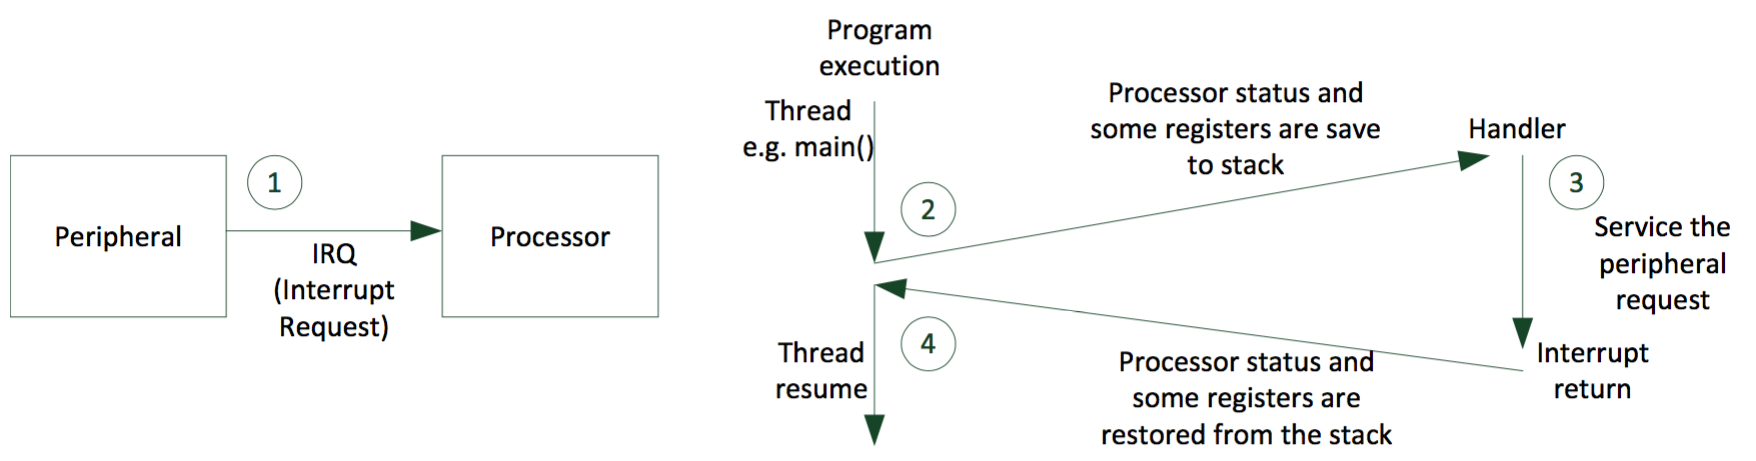
\includegraphics[width=\textwidth]{interrupt_basics}
    \caption{Operation of an Interrupt}
    \label{interrupt_basics}
\end{figure}

Interrupts are usually generated by peripherals within the embedded device. These events are used to signal a change in the peripheral state, such as receiving data from a communications interface. Other interrupts signal error conditions or are used to recover from bad processor states caused by disallowed operations within the main program. Many interrupts can be directly triggered by the user's code to perform operations with a higher priority than the main thread. 

Every interrupt has a hardware number designation. An interrupt's number indicates its hardware priority and is used to index into the \textit{Vector Table}. The Vector Table for a processor usually exists at the beginning of the system address space and is a list of memory addresses associated with the handling of a specific interrupt. For example, the RESET vector's (in actuality a RESET interrupt) location in the Vector Table is directly at the beginning. This results that the first few instructions that the processor executes after power-on are a load and branch to the reset handling code. 

Whenever an interrupt is triggered, the processor hardware uses the interrupt number to index into the Vector Table to find the memory address of the interrupt handling code. The processor hardware saves the current register and stack state before branching to the loaded handler address. After the routine completes, any original state is restored, and the main program executes almost as if it was never interrupted. 

Figure \ref{vector_table} (peripheral reference manual pages 217-219) shows the documentation for the STM32F072 Vector Table. The Vector Table is located within the startup assembly code for the processor. It defines human-friendly names used to designate functions as the appropriate interrupt handling code. When compiling and linking, the toolchain places the address of these functions within the Vector Table data.  

\begin{figure}[]
    \centering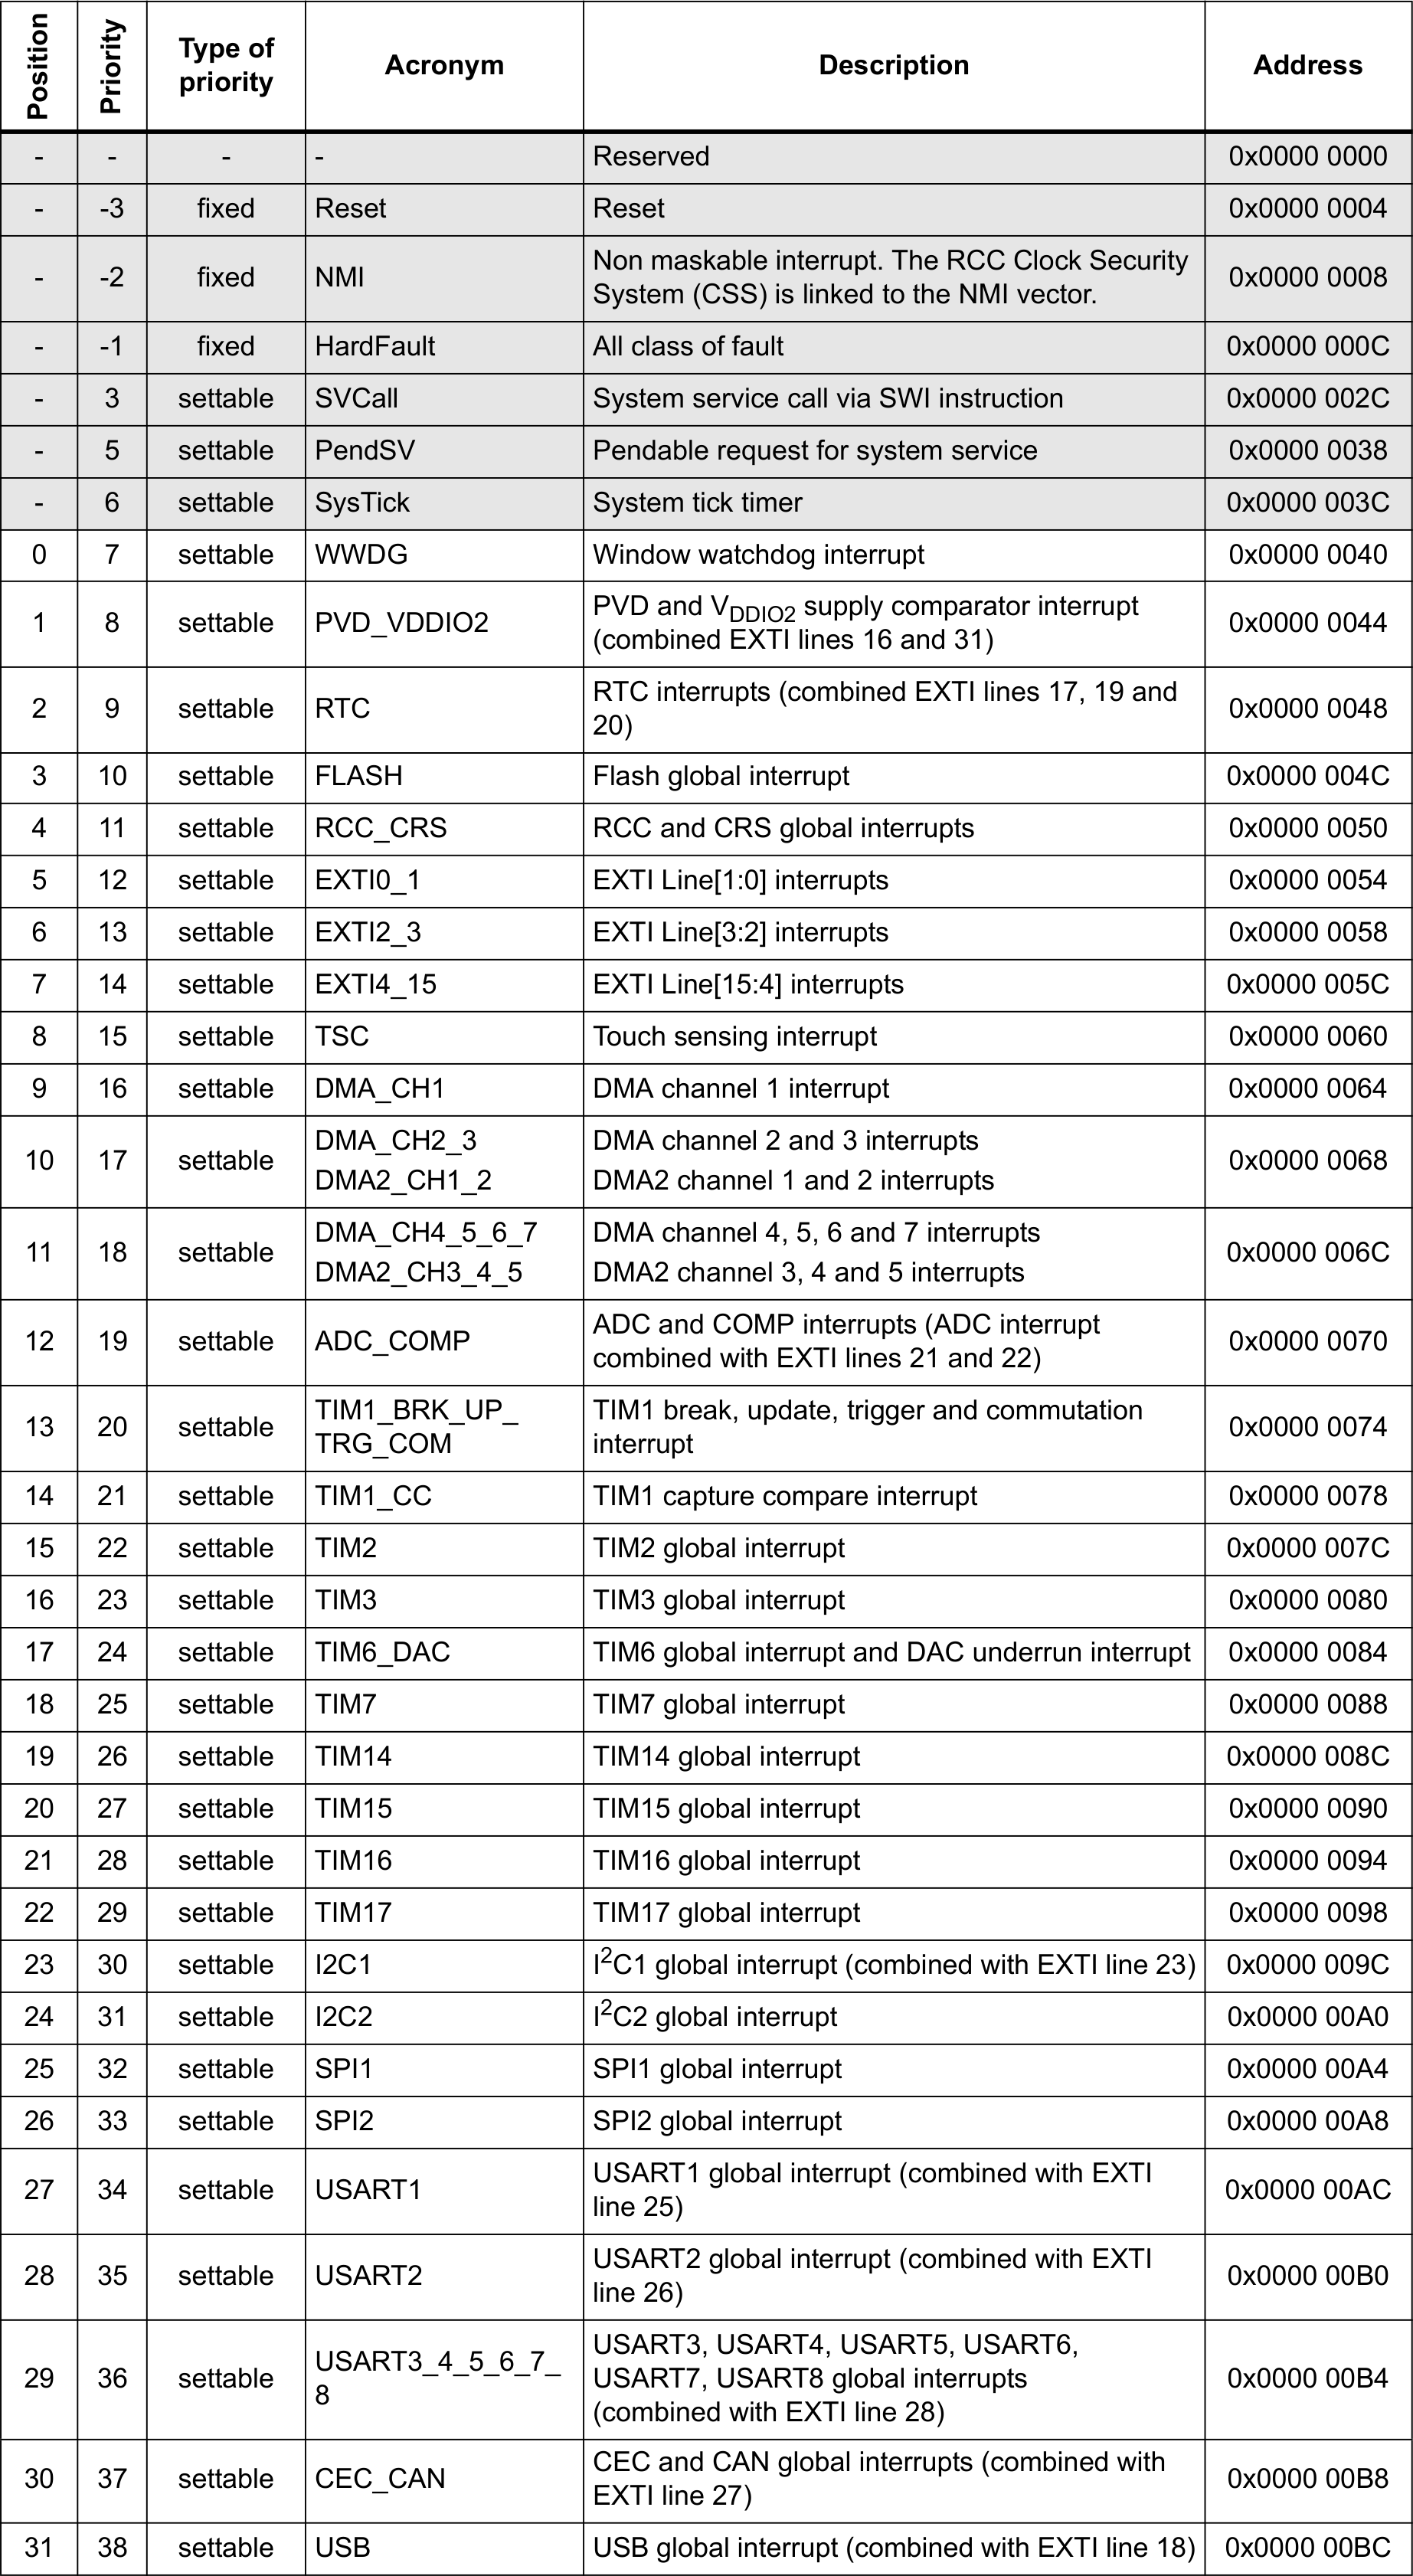
\includegraphics[height=\textheight]{vector_table}
    \caption{STM32F072 Vector Table}
    \label{vector_table}
\end{figure}

% REVISE: how to find stuff in files will be handled later, whats in each file, remove the info here
% Talk about negative priorities and what can/cant be masked
% Talk about special-purpose interrupts

The Kiel:MDK toolchain and HAL library have already defined a few interrupt handlers within the \textit{stmstm32f0xx\_it.c} file located under the \textit{Application/User} {\textmu}Vision project folder. The device startup code and Vector Table implementation are located in the \textit{startup\_stm32f072xb.s} file within the \textit{Application/MDK-ARM} directory. 

% interrupt terminology
% what can generate interrupts
%   avaliable interupts in the stm32
%   location of interrupt handlers in MDK


\section{Managing System Interrupts}
%Figure \ref{peripherals}
Figure 2.3 in the previous lab showed a block diagram of the peripherals within an STM32F072 device. Considering that many of these peripherals can generate interrupts, there are a large number of possible sources that the system must recognize and manage. Some peripherals share interrupts, and within a single peripheral there may be multiple trigger conditions.  

Because of the large number of possible interrupt sources, there must be a way to enable, sort and otherwise manage them. Because interrupts are tightly bound to the operation of the actual processor core, within the ARM Cortex-M0 itself, exists the Nested Vectored Interrupt Controller (NVIC).

\subsection{The Nested Vectored Interrupt Controller}
The primary responsibilities of the NVIC are to enable and disable interrupts, indicate requests waiting to be serviced, cancel pending interrupt requests, and set how multiple interrupts interact through configurable priorities. A simplified block diagram of the NVIC is shown in figure \ref{nvic}.
    
%(Graphic with NVIC taking processor-external signals and controlling the PC and register file)
\begin{figure}[h]
    \centering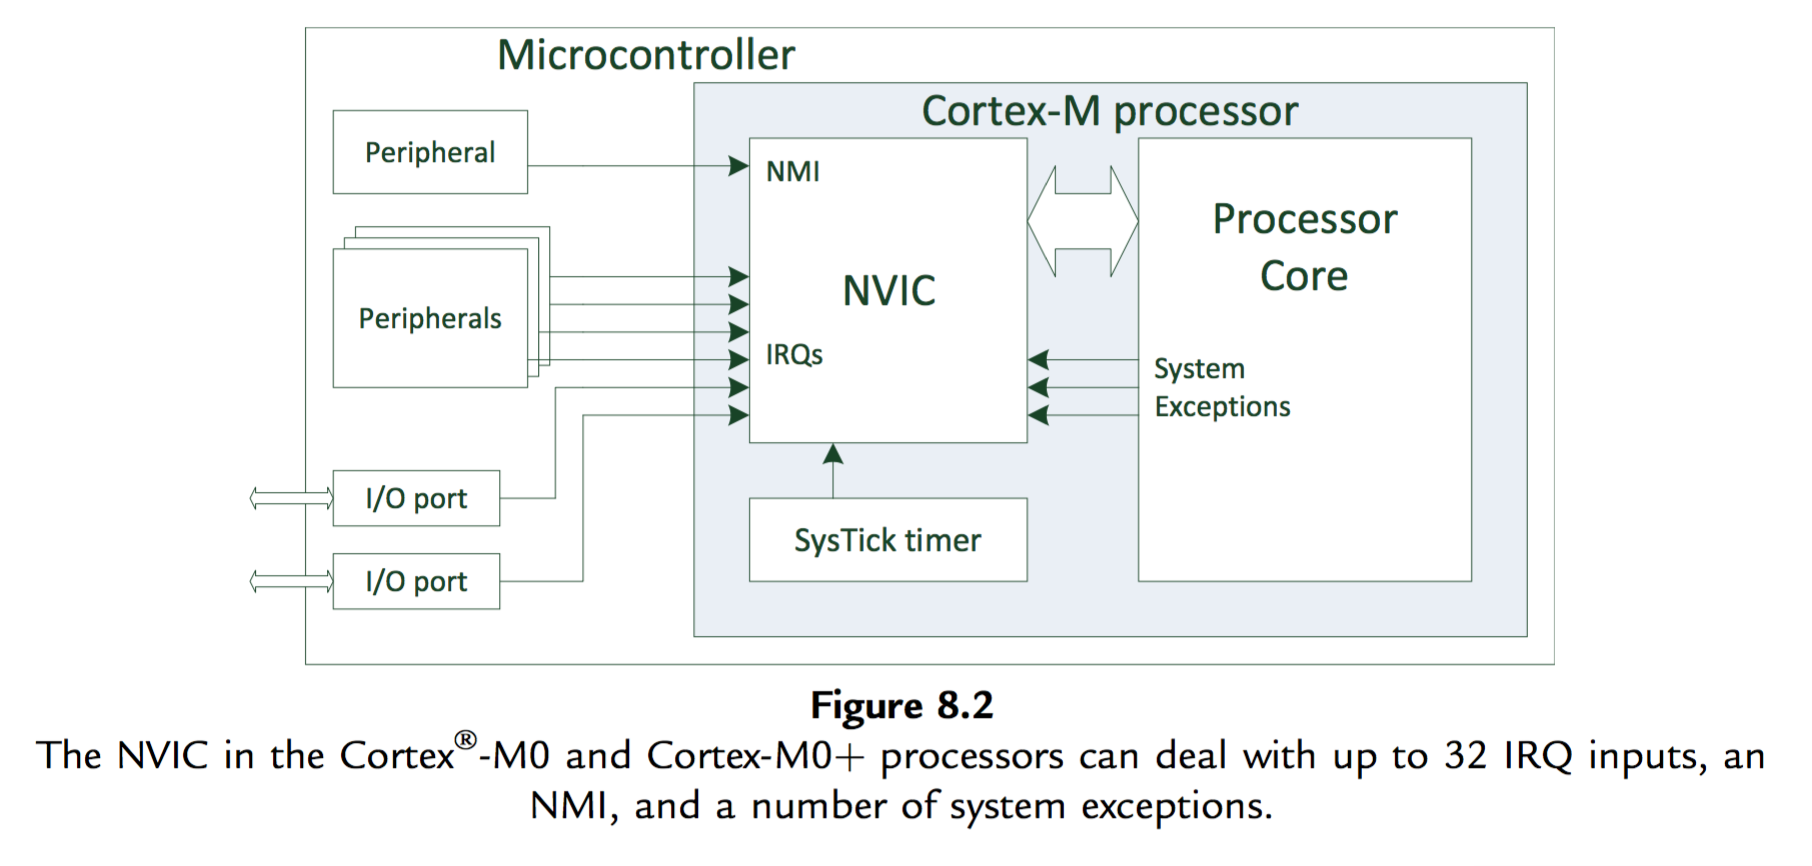
\includegraphics[width=\textwidth]{nvic}
    \caption{The Nested Vectored Interrupt Controller}
    \label{nvic}
\end{figure}

Depending on the type of ARM core present within a device, the NVIC features different capabilities. Within a Cortex M0 device such as the STM32F0, the peripheral only contains the few types of control registers. Because the NVIC is a ARM-core peripheral it is documented in the ARM core and programming manual not the STM32F0 peripheral reference manual. Additionally the structure and register definitions are located in the \textit{core\_cm0.h} file and not in the \textit{stm32f072xb.h} like the other peripherals.  

Open the core programming manual and go to page 71. Beginning here is the register documentation for the NVIC peripheral. A summary of the NVIC registers is as follows:

\begin{itemize}
    \item \textbf{Interrupt set-enable register (ISER)}
        \begin{itemize}
            \item The ISER register enables interrupts and indicates which are enabled.
            Writing a `1' to a bit enables the matching interrupt, this register is ``read and set only,'' meaning that attempts to clear bits are ignored. 
        \end{itemize}
    \item \textbf{Interrupt clear-enable register (ICER)}
        \begin{itemize}
            \item The ICER register disables interrupts.
            This register uses a write to clear scheme. Writing a `1' to a bit disables the matching interrupt. This register is ``read and write-one-clear only,'' meaning that attempts to clear bits are ignored. 
        \end{itemize}
    \item \textbf{Interrupt set-pending register (ISPR)}
        \begin{itemize}
            \item The ISPR shows which interrupts are pending, and can manually force interrupts into a pending state. 
        \end{itemize}
    \item \textbf{Interrupt clear-pending register (ICPR)}
        \begin{itemize}
            \item The ICPR shows which interrupts are pending, and can manually clear pending status for an interrupt. This can be used to cancel an interrupt request before the interrupt handler is launched.
        \end{itemize}
    \item \textbf{Interrupt priority registers (IPR0-IPR7)}
        \begin{itemize}
            \item These registers configure the priorities for each interrupt. 
            \item Each IPR register contains four 8-bit regions dedicated to configuring the priority of a specific interrupt. The NVIC within the STM32F0s only has the uppermost two bits from these regions implemented, giving four possible configurable priority levels.            
        \end{itemize}
\end{itemize}

\subsection{Interactions Between Multiple Interrupts}
As the number of enabled interrupts within a system increases, the possibility of an interrupt request occurring during the handler of another becomes likely. Because of this, there must be a deterministic way of dealing with inter-interrupt interactions. The NVIC solves this problem with a system of both software configurable and fixed hardware interrupt priorities. Depending on these priority settings there are two possible outcomes for multi-interrupt conditions. Figure \ref{tailChain_nesting} shows a graphical representation of each mode of operation.

\begin{figure}[]
    \centering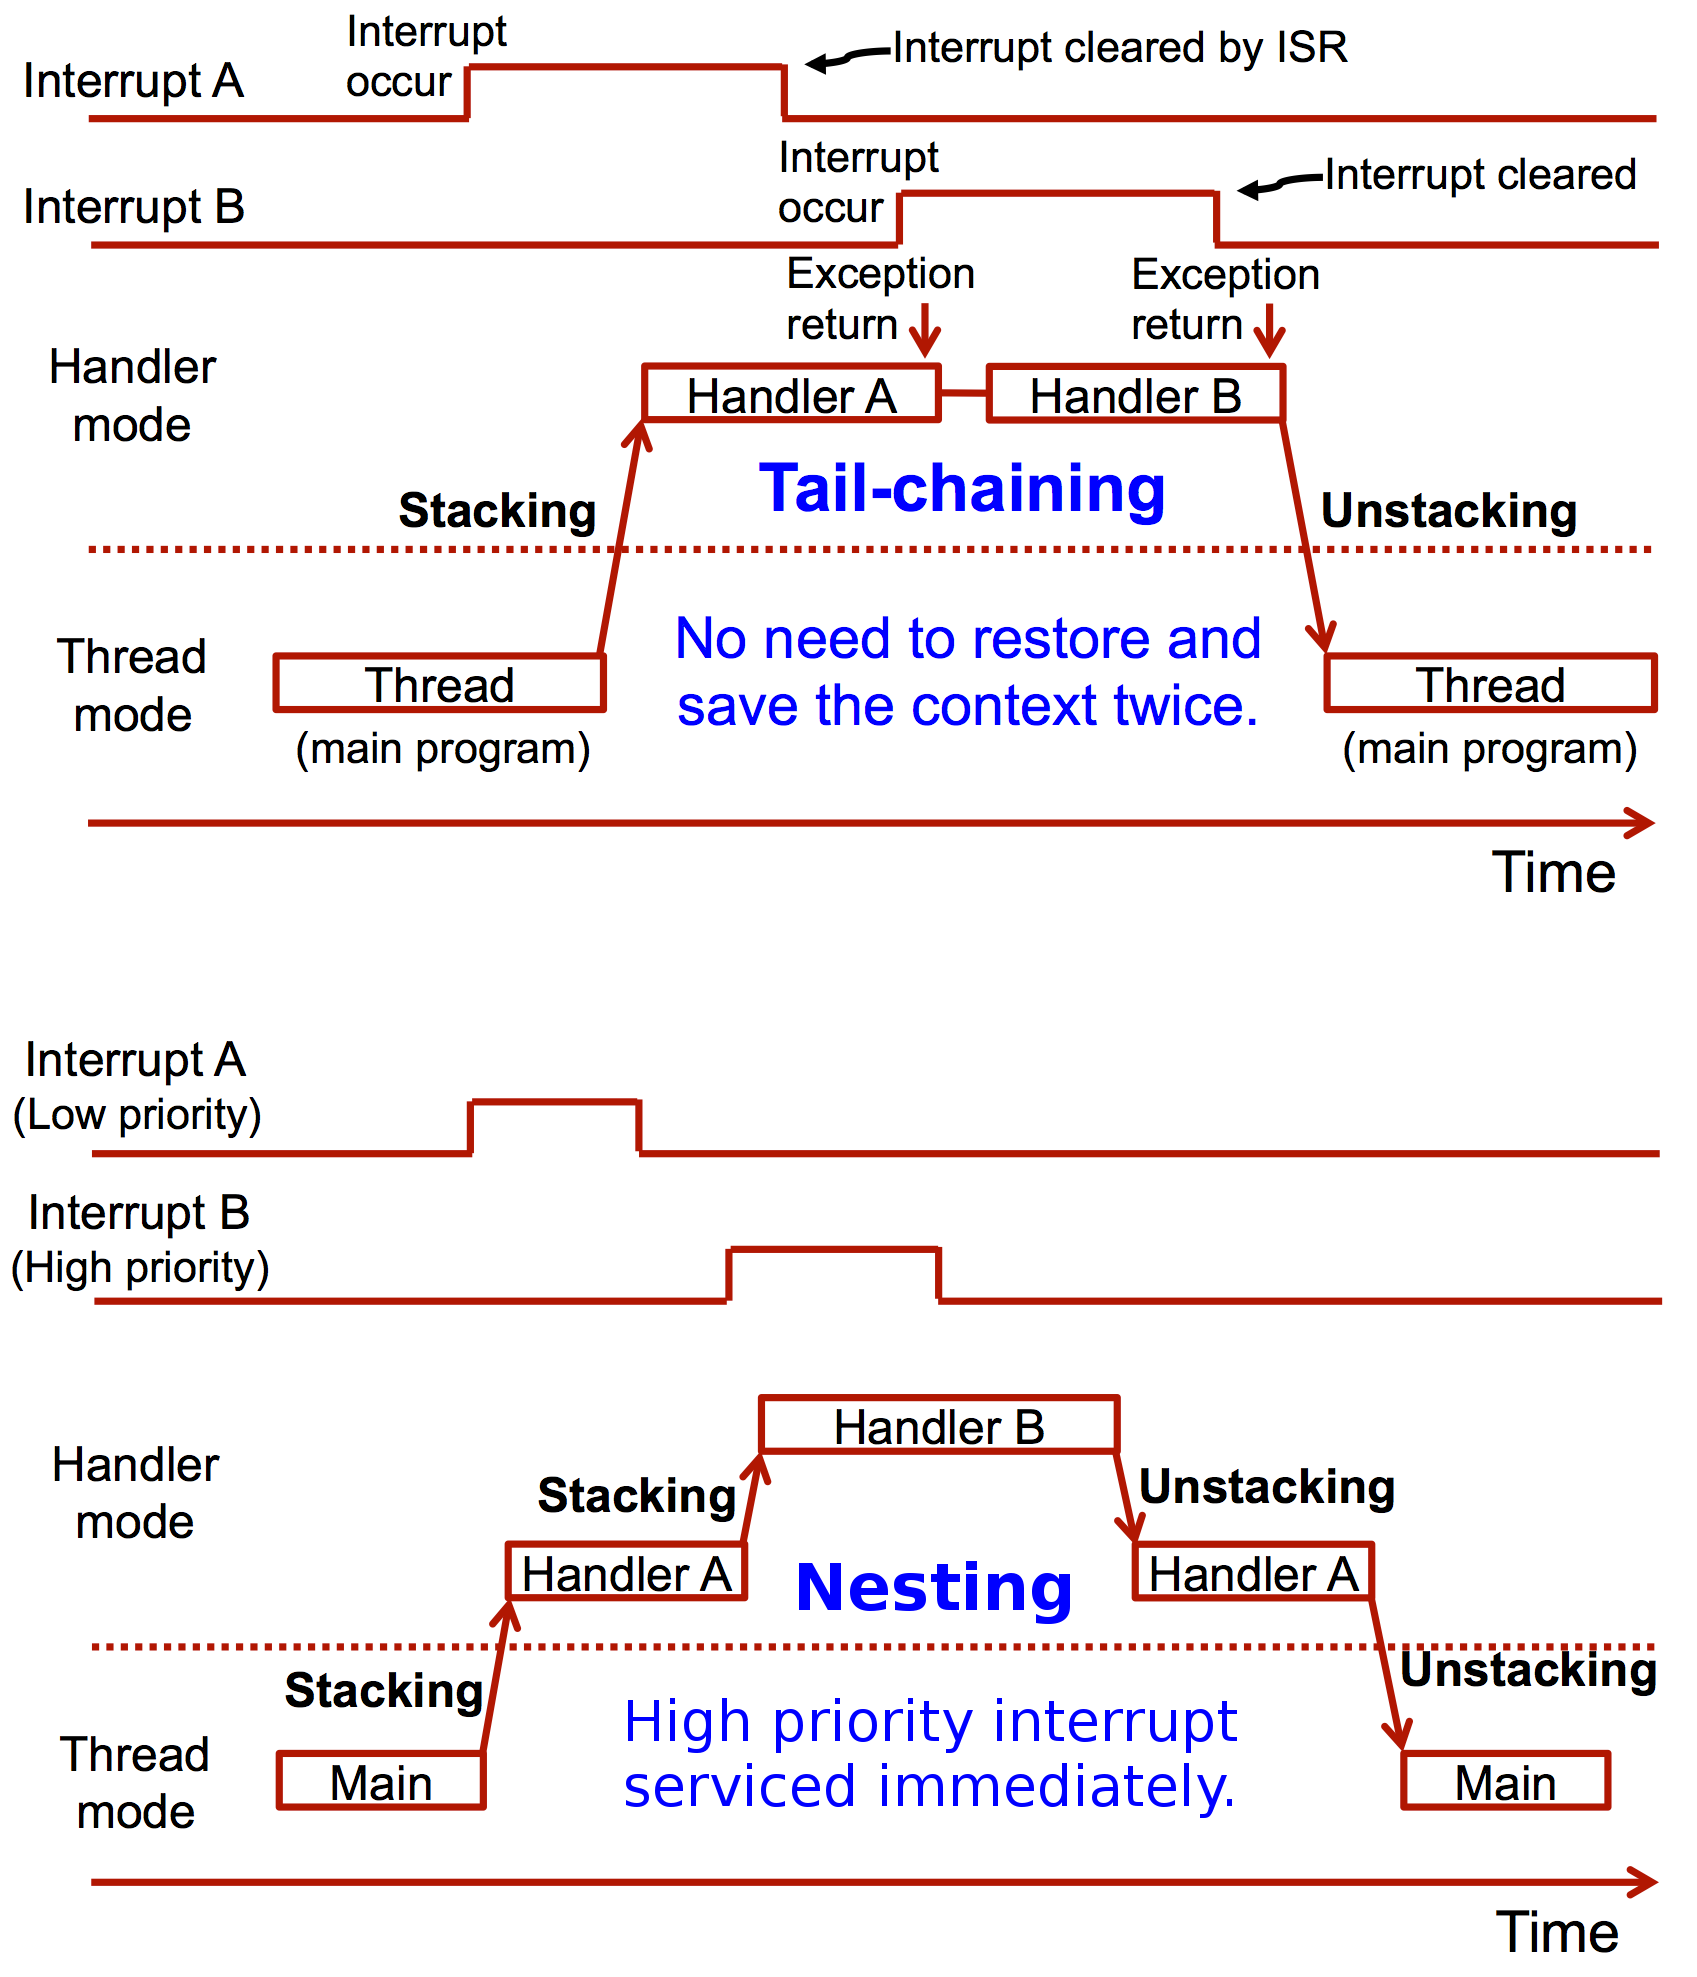
\includegraphics[width=0.6\textwidth]{tailChain_nesting}
    \caption{Multi-Interrupt Ordering Modes}
    \label{tailChain_nesting}
\end{figure}

\subsubsection{Tail-Chaining}
Some embedded processors have only a built-in hardware ordering between interrupts. In these systems, if multiple interrupt trigger concurrently or during a handler, they are executed one after each other according to the hardware priority. In this mode known as \textit{tail-chaining}, interrupt handlers are never interrupted. Tail-chaining can use a simple save and restore mechanism for transitioning from the main thread but has the disadvantage of allowing a rapidly triggering or long running interrupt high on the hardware priority to ``starve'' or prevent lower interrupts from executing. 

The NVIC will tail-chain interrupts configured to the same software priority within the IPR registers. If multiple interrupts with the same software priority become pending at the same time, the built-in hardware ordering will determine the next handler to launch.

\subsection{Interrupt Nesting}
Unlike systems having only hardware interrupt priorities, the NVIC allows important interrupts to interrupt lower priority handlers. This process called \textit{nesting} requires a more complex context-switch mechanism but otherwise works identically to how interrupts pause execution of the main application thread. 

Allowing nested interrupts introduces some complications. Some interrupt tasks can not be interrupted without losing or corrupting data. An example of this are interrupts which move data between communication peripherals. Many of these have limited buffer space and will overwrite data if the interrupt execution is delayed or paused for too long. 

Much of this can be handled by setting the priorities between interrupts properly. However, in some cases, it may be appropriate to \textit{mask} or temporarily disable other interrupts during critical sections of code. The NVIC has capabilities to mask specific interrupts, and larger relatives such as those in the Cortex M3 devices can mask interrupts by priority level. When an interrupt is masked, it is still able to enter the pending state; this allows the NVIC to evaluate and launch the appropriate handlers once the masks has been removed.
 

 
\subsection{Using CMSIS Libraries to Configure the NVIC}
Similar to ST Microelectronics which publishes the HAL library for STM32F0 peripherals, ARM Ltd provides the \textit{cortex microcontroller software interface standard} (CMSIS) library which controls Cortex M0 peripherals. 

Although the NVIC has a fairly simple register interface modifying interrupts can become a complicated task to do safely. One of the main issues with directly modifying NVIC registers is that if an interrupt were to occur during the process, there is a possibility of corrupting or overwriting the register state.  

Because the NVIC is within the ARM core its interface remains consistent across multiple vendors devices. This is beneficial because the CMSIS library functions are usually available regardless of the specific chip manufacturer. 

Within the exercises in these labs you have the choice of controlling the NVIC through the CMSIS library or register access. These CMSIS functions are located after the peripheral structure and register definitions in the \textit{core\_cm0.h} file. 


%\begin{figure}[h]
%    \centering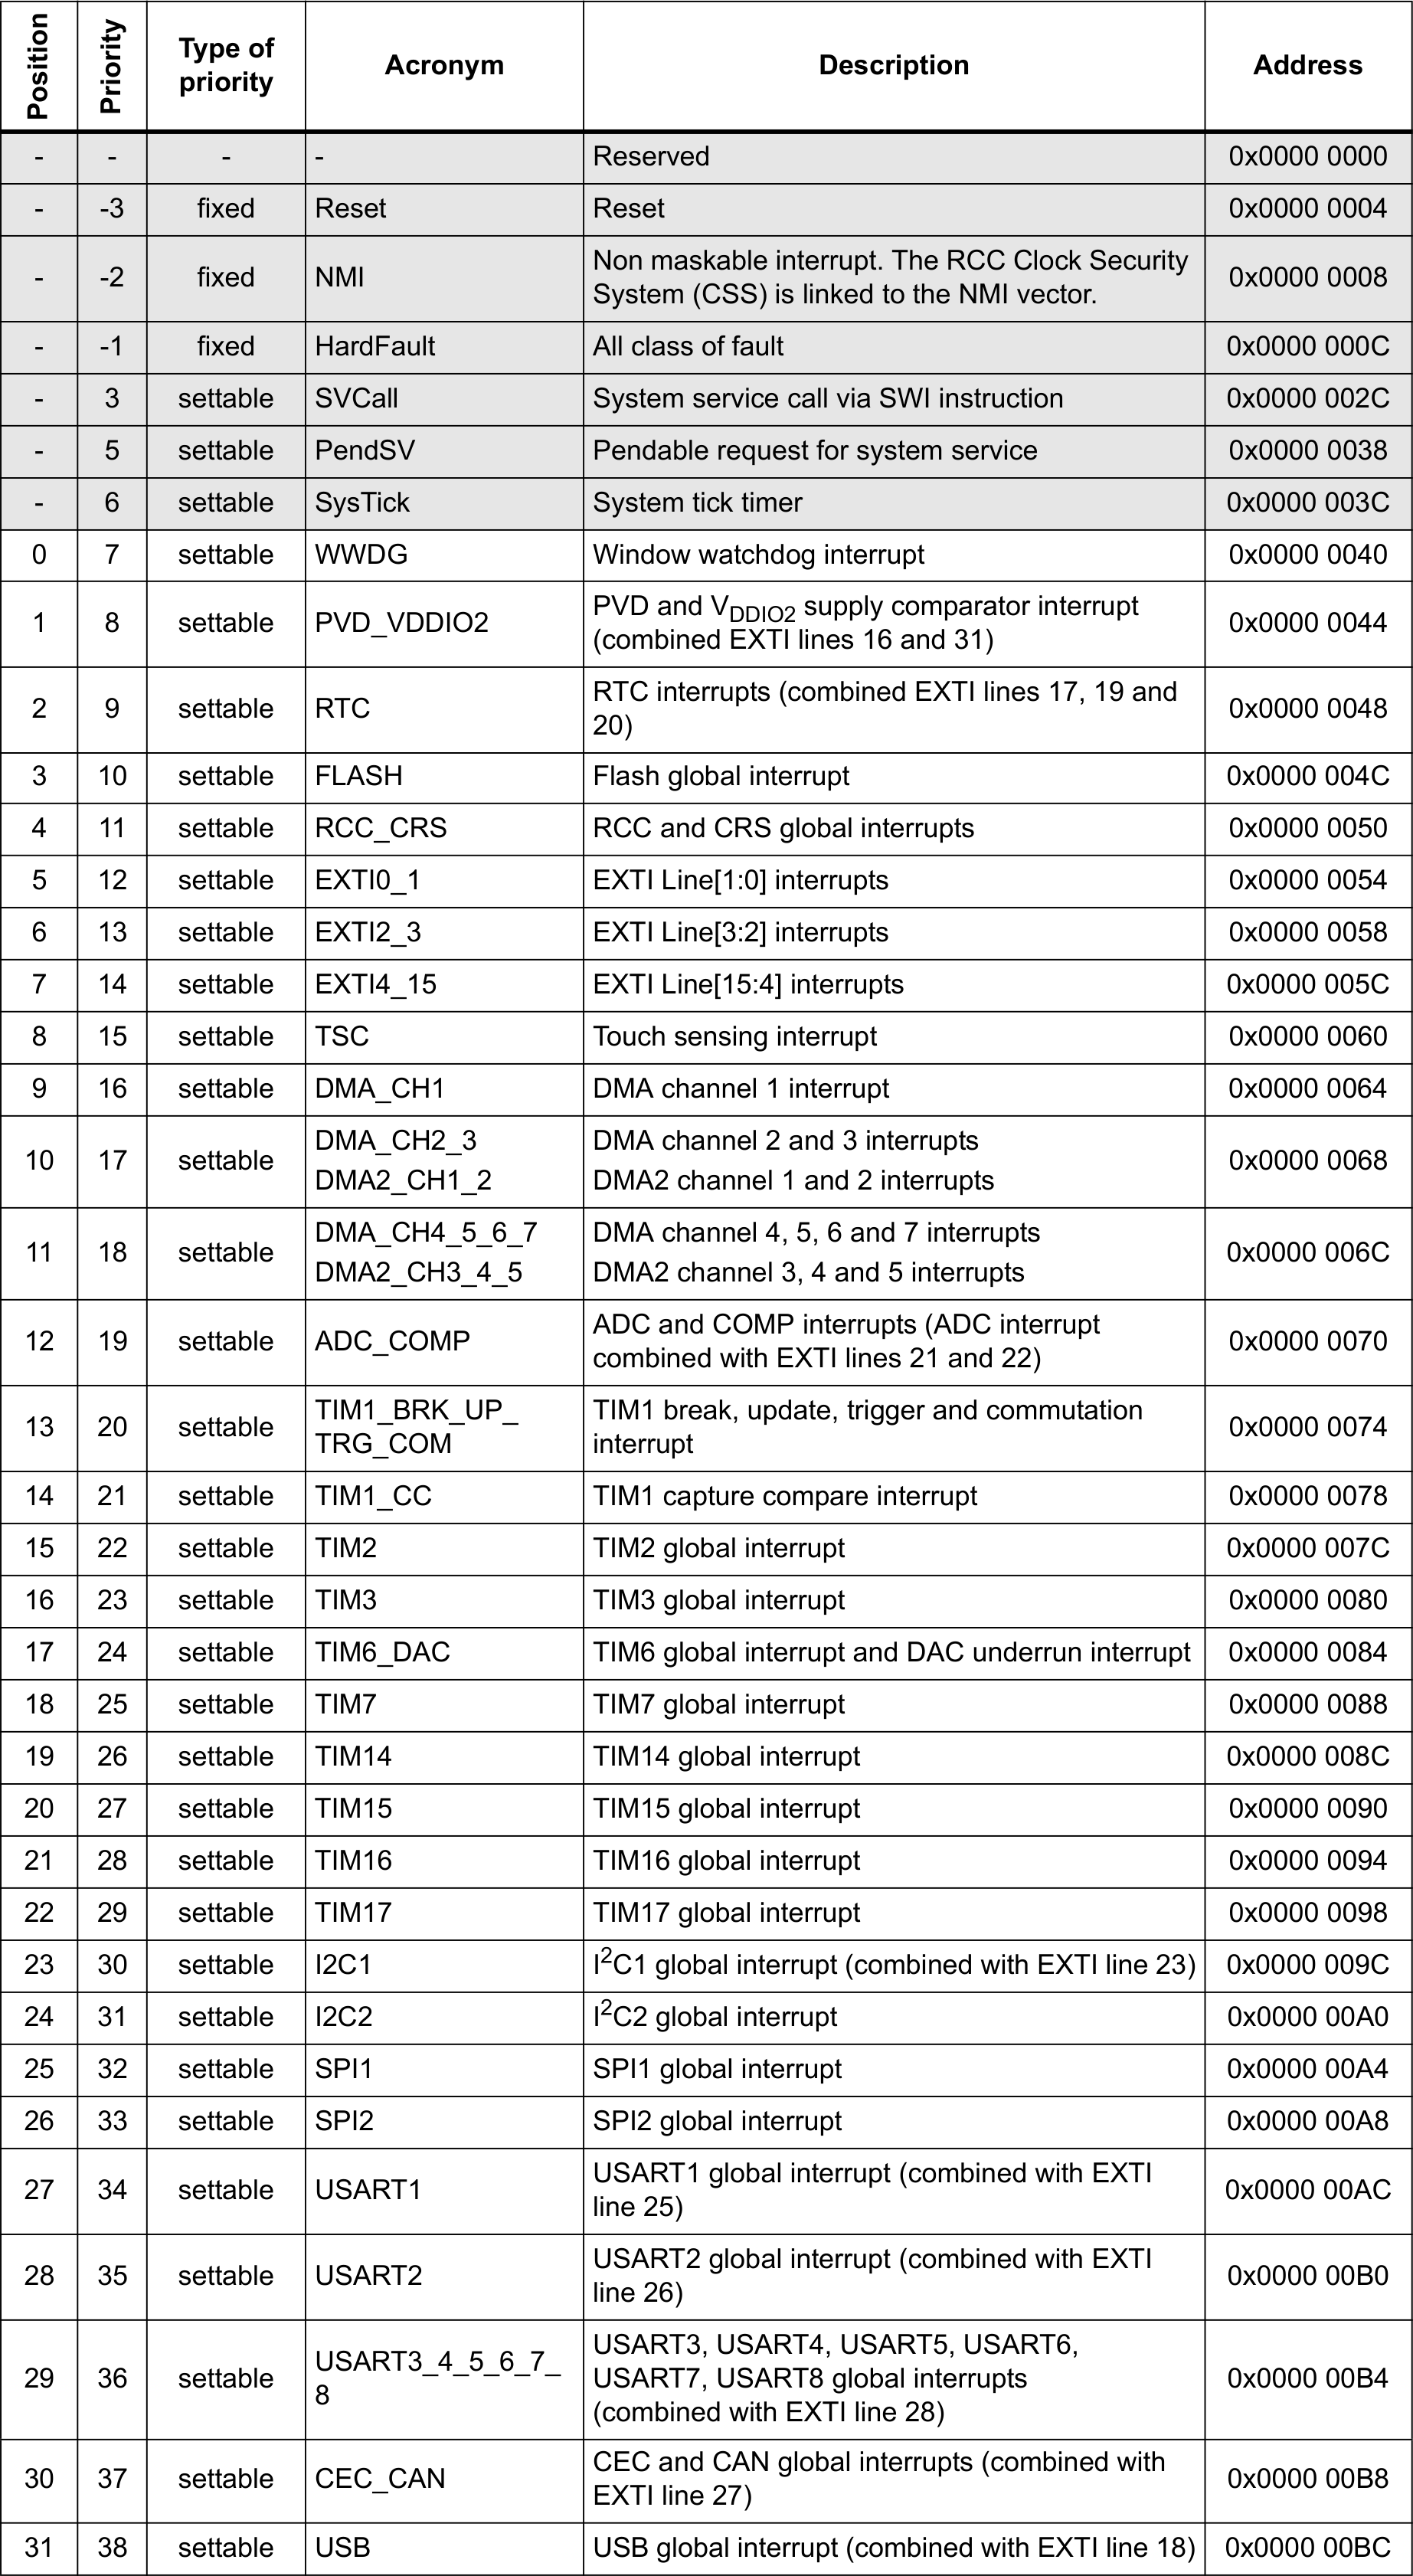
\includegraphics[height=\textheight]{vector_table}
%    \caption{STM32CubeMX new project window with filters applied}
%    \label{cube_newProj}
%\end{figure}

% Location in system
% Features & Capabilities
% ``Nesting'' vs ``Tail-Chaining''
% Interrupt Priorities, setting priorities
% Starvation & Priority inversion

\section{Triggering Interrupts With External Signals}
% Polling vs Interrupt/Idle Sleep

In the previous lab, we used a button press on the Discovery board to toggle between two LEDs. To do this, we repeatedly checked the button state in the infinite loop of the main application. This method of detection is called \textit{polling}. Polling has the advantage that the repetitive and periodic checking enables tricks such as software debouncing. However it has the disadvantage of using a significant amount of processor cycles even when the device could otherwise be idle. 

In some embedded systems such as the Discovery board, wasting energy on polling is not a significant challenge as continuous power is readily available. However, many battery-powered systems need to reduce the power consumption by any means possible to prolong the battery life.

One method of avoiding continuous polling is to utilize the interrupt system of the processor to monitor and detect changes in a pin's state. With the ability to do this it becomes possible to place the device into a low-power mode when no other processing is required. 

The exercises in this lab will be using the ``Wait for Interrupt'' (WFI) assembly instruction which puts the processor into ``sleep'' mode. This is the least drastic of the low-power modes that the STM32F0 offers. In this state, the ARM processor is stopped, but all memory and peripherals operate normally. Any hardware interrupt has the capability to start the processor again; once the interrupt handler exits, the main program will continue the main application thread. Other low-power modes selectively shutdown additional peripherals, system oscillators, and power circuitry. These modes are more limited in the methods available to wake them up, and some of them lose device state.  

\subsection{Extended Interrupts and Events Controller} \label{exti}

The \textit{Extended Interrupts and Events Controller} (EXTI) is the peripheral that allows non-peripheral sources to trigger interrupts. While typically used to generate interrupts from the GPIO pins of the device, it also has the ability to monitor various internal signals such as the brownout protection circuitry. (low-voltage shutdown)

The EXTI documentation begins on page 219 of the peripheral reference manual. Similar to the NVIC,  bits within the EXTI registers do not feature names suggesting the signals they control. The documentation within \textit{functional description} section on the peripheral describes the mapping between EXTI event ``lines'' or input sources and the control bits.  

\begin{itemize}
    \item \textbf{Interrupt mask register (EXTI\_IMR)}
    \begin{itemize}
        \item The IMR register ``unmasks'' or enables an input signal to generate one of the EXTI interrupts.
    \end{itemize}
    \item \textbf{Event mask register (EXTI\_EMR)}
    \begin{itemize}
        \item Processor events are similar in design to interrupts but do not cause program execution to branch to separate handler code. Events are typically used to wake the processor from low-power modes. The EMR enables input signals to generate processor events. 
    \end{itemize}
    \item \textbf{Rising trigger selection register (EXTI\_RTSR)}
    \begin{itemize}
        \item All external (pin) interrupts are edge-sensitive. This means that they only generate interrupt requests at the transitions from one logic state to another. The RTSR enables a rising/positive-edge trigger for a pin.
    \end{itemize}
    \item \textbf{Falling trigger selection register (EXTI\_FTSR)}
    \begin{itemize}
        \item The FTSR enables a negative/falling-edge trigger for a pin. The EXTI allows both rising and falling triggers to be enabled for an input.  
    \end{itemize}
    \item \textbf{Software interrupt event register (EXTI\_SWIER)}
    \begin{itemize}
        \item The SWIER register allows the user to manually trigger any of the interrupt or event conditions within the EXTI as long as the matching bits in the IMR or EMR registers are also set. 
    \end{itemize}
    \item \textbf{Pending register (EXTI\_PR)}
    \begin{itemize}
        \item  The pending register indicates whether an trigger event has occurred on an input signal since the pending flag was last cleared. As long as the corresponding interrupt is enabled the EXTI interrupt handler will be repeatedly called unless the corresponding pending flags are cleared. 
    \end{itemize}
\end{itemize}

% What is the EXTI Peripheral 
% Main registers and operation


\subsection{Pin Multiplexing with the SYSCFG} \label{syscfg}
% SYSCFG Muxes
Although the STM32F0s have the ability to generate external interrupts on almost any pin, there are only 16 available input lines to the EXTI. Because of this, there are a series of pin multiplexers selecting the pins that connect to the limited EXTI inputs.  

These multiplexers are controlled by the \textit{System Configuration Controller} (SYSCFG) peripheral. The SYSCFG deals primarily with signal routing and controls data transfer between peripherals and memory, remapping portions of memory, and some high-power communication modes. 

Figure \ref{exti_mux} shows the SYSCFG pin multiplexers used by the EXTI. These multiplexers group external pins by their orderings within the GPIO peripherals. For example, PA0, PB0 ... PF0 are grouped on a single multiplexer with the output routed to the EXTI0 input. Because only a single pin from a group can be used, pins need to chosen such that they do not conflict with each other when using multiple external interrupts.

The multiplexers are configured by the EXTICRx registers within the SYSCFG peripheral. The register maps for these begin on page 177 of the peripheral reference manual. 

\begin{figure}[]
    \centering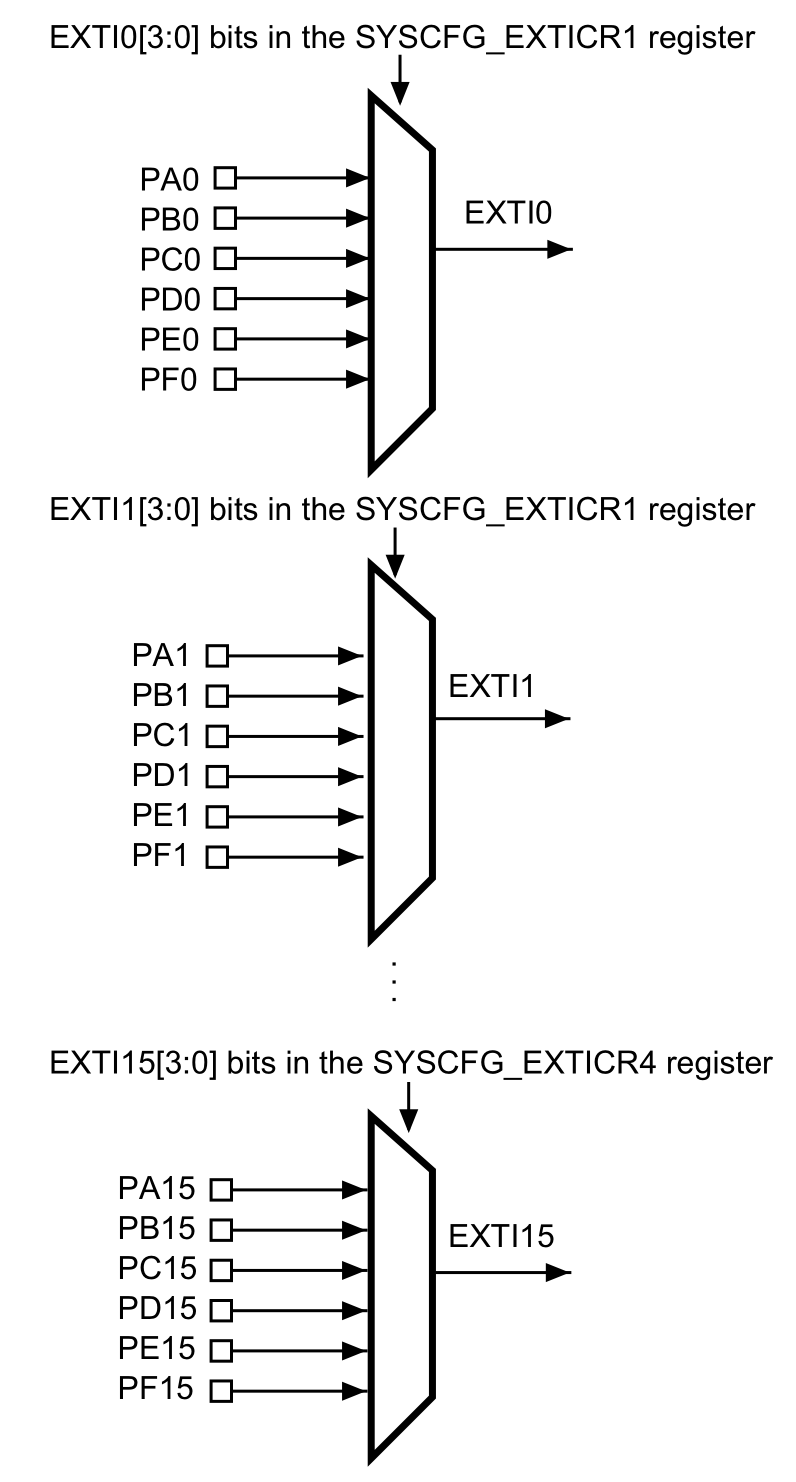
\includegraphics[height=0.5\textheight]{exti_mux}
    \caption{SYSCFG/EXTI Pin Multiplexers}
    \label{exti_mux}
\end{figure}

\section{Working With Interrupts} 
The examples in this section of the lab demonstrate the process of setting up an interrupt for the \textit{Universal-Synchronous-Asynchronous-Transmitter} (USART). You are not expected to know how the USART operates, that will be the topic for a later lab, but understand that it is a communications peripheral with has the capability of generating an interrupt after receiving a full byte of data. 

\subsection{Enabling and Setting Priorities for an Interrupt}


\subsubsection{Configuring a Peripheral to Generate Interrupts} \label{periph_setup}
Most peripherals have multiple conditions that can trigger an interrupt. These conditions may signal different events or error states that may occur in the operation of the peripheral. Usually all interrupt-based features within a peripheral are disabled by default, this allows the user to enable only the conditions that they wish to manage in their interrupt handler. 

\begin{example}[Enabling the USART RXNE Interrupt]
     In this example we'll be enabling the \textit{receive register not empty interrupt} (RXNE) which ``fires'' or triggers whenever new data arrives and is waiting to be processed. 
    
    Open the peripheral reference manual to page 720 and examine table 26.7 \textit{USART Interrupts.} This table lists all of the events that can trigger the USART interrupt. Because these events must share a single interrupt handler, they set status bits which are used to determine what event needs to be managed. The table also lists the control bits that need to be set to enable the interrupt for each specific event.
    
    From table 26.7, we can see that we need to set the \textit{RXNEIE} bit to enable the receive interrupt condition. This bit is located within the \textit{Control Register 1} (CR1) of the USART peripheral. The following line of code configures USART1 to signal an interrupt request whenever data is received
    
    \ilcode{USART1->CR1 |= USART\_CR1\_RXNEIE;   // Enable RX interrupt in USART}
    \smallskip
\end{example}

\subsubsection{Enabling the Interrupt within the NVIC} \label{nvic_setup}
In the previous example we configured the USART to generate an interrupt request whenever new data arrives. However, unless the NVIC is also configured to allow the interrupt it will simply ignore the request. 

Using the CMSIS library functions in \textit{core\_cm0.h} simplifies configuring the NVIC. These functions identify the interrupt to be modified by a number representing its index in the Vector table. These numbers have conveniently been given defined names in the \textit{IRQn\_Type} enumeration within the \textit{stm32f072xb.h} file.  

Because the NVIC within the STM32F0 has two configuration bits for each interrupt's priority, there are four software priority levels available. The CMSIS library functions accept a numeric value in the range of [0-3] as allowed priority levels. The lower the priority value given, the higher the actual priority assigned to the interrupt by the NVIC. 

\begin{warning}
    Remember that the highest software priority level for the NVIC is 0, the lowest is 3. The hardware priorities also follow a similar scheme with lower indexes in the Vector table having higher priority. 
\end{warning}

% talk about NVIC numbers in the stm32f072xb.h

% talk about avaliable priority levels
% 3- low
% 2 - medium
% 1 - high
% 0 - very high (higest)

\begin{example}[Configuring the NVIC]
   First we need to look up the appropriate interrupt number, preferably by a defined name in the \textit{stm32f072xb.h} file. Afterwards we can pass it to the \texttt{NVIC\_EnableIRQ()} function to enable the interrupt.
   
   \ilcode{NVIC\_EnableIRQ( USART1\_IRQn )}
    
    After enabling the interrupt, we need to set the priority. Since the USART may be receiving a stream of data, we will need some buffer unless it is possible to process each byte as it arrives. Unfortunately the USART's receive register can only hold a single byte at a time, and if new data arrives before we have read the previous byte, it will be overwritten. This means that we will have to do the buffering ourselves, and depending on the speed that the USART is configured to use, we may not have time to wait around until it becomes convenient to move the data.
    
    This probably means that we will want to give the USART a higher priority than many of the other interrupts. The following code snippet configures the USART interrupt to high priority.  
    
    \ilcode{NVIC\_SetPriority(USART1\_IRQn, 1 );  // Configure to high priority}
    \smallskip
\end{example}
\subsection{Setting up the Interrupt Handler}  \label{handler_setup}
Once the interrupt has been enabled within both the peripheral and NVIC, it is time to define a region of code as the appropriate handler. 

The MDK:ARM toolchain includes a set of function names used for interrupt handlers. These are automatically referenced by the Vector table when compiling and linking. Declaring a function using one of these defined names automatically makes it into an interrupt handler.

These names are defined with the Vector table in \textit{startup\_stm32f072xb.s}. Your interrupt handlers must be declared to accept no arguments and have no return value. 

Most peripherals have a status register containing flag bits for pending interrupt requests. However, even in those without dedicated registers, most interrupts set status flags within their peripheral. These flags are used to generate interrupt requests. Typically you will need to manually clear the matching status bit for the interrupt condition you are handling. Otherwise, the interrupt will continuously repeat because the request is never acknowledged as completed. 

\begin{warning}
    Always check the conditions for clearing status flags in the reference manual!
    
    Many status registers are cleared by writing a one to the bit position. Others are read-only and must be cleared through other methods. 
    
    Some peripherals such as the USART automatically clear some status flags. For example, explicitly clearing the receive interrupt flag in a USART is unnecessary since it self-clears whenever the receive register is read. 
\end{warning}

% talk about vector table defining names in startup_stm32f072xb.s

\begin{example}[Writing the USART Interrupt Handler]
    In the \textit{startup\_stm32f072xb.s} file, we can see the implementation of the Vector table. This table lists a series of (mostly) unimplemented function names that are linked by the toolchain whenever the appropriate interrupt request is signaled from the NVIC. 
    
    Looking down the table, we can find the name for the USART1 handler to be ``USART1\_IRQHandler'' We can use this name to define a function anywhere within the code project. Typically, interrupt handlers are placed either within the interrupt specific code file \textit{stm32f0xx\_it.c}, main.c, or files containing the peripheral's driver.  
    
    Figure \ref{usart_isr} shows a completed interrupt handler for the USART1. It begins by checking all enabled conditions to find the one triggering the interrupt, clears the condition flag, and performs some action. 
    
    \code{./Files/usart_isr.c}{Example USART RXNE Interrupt Handler}{usart_isr}
    
\end{example}


% Setup and enable an interrupt
%   depends on peripheral
%       enable trigger/request in peripheral
%       set priority and enable in NVIC
% Handler
%   Use default or override function stub

% Saleae Logic User Guide 
% (PDF) http://downloads.saleae.com/Saleae+Users+Guide.pdf
% (Online) http://support.saleae.com/hc/en-us/sections/201990573-saleae-users-guide

\section{Lab Assignment: Writing Interrupt-Based Code}
The following exercises explore basic concepts of interrupt-driven programming, peripheral-interrupt configuration, and how priorities order multiple interrupts. After completing these tasks, make sure to show the lab assistant! Most of your points for the lab will come from demonstrating your solutions.

\subsection{Modifying an Existing Interrupt}
% Toggle LEDs in SysTick ISR
In this exercise, you will modify the SysTick timer interrupt to perform some user operations. In the project template that STMCube generates, the SysTick timer is already configured as part of the HAL library initialization. 

The SysTick peripheral is a simple countdown timer which begins at a software set value. Once the value of the timer reaches zero, an interrupt is triggered, and the timer resets. By default, the HAL configures the SysTick interrupt to occur once every millisecond. The interrupt handler is located within the \textit{stm32f0xx\_it.c} file.  

\subsubsection{Adding Code to the SysTick Interrupt}

\begin{enumerate}
    \item Locate the SysTick interrupt handler and write a simple application which blinks or flashes LEDs in the handler.
    \begin{itemize}
        \item Choose something reasonable, but have fun. Your code can be a single flashing LED or a complex multi-color pattern. 
    \end{itemize}
    \item Configure used GPIO pins in the main application. Don't place run-once code such as initializations in the handler.
    \item Your modified SysTick handler will be called every millisecond. Because of this periodicity, you can count the number of iterations as a timing basis.  
    \begin{itemize}
        \item For example, toggling an LED every 200th time the handler is called results in 200 ms between blinks. 
        \item You will need to use either a volatile global variable or local-static variable to store interrupt count. 
        \item \textbf{Do not use delay functions in the interrupt handler.}
    \end{itemize}
    \item Remove any existing code within the infinite loop of the main function. 
    \begin{itemize}
        \item We want the processor to go to sleep when not executing an interrupt handler.
        \item Place a call to the \texttt{\_\_WFI()} function in the infinite loop. 
        \begin{itemize}
            \item This function executes an assembly \textit{wait for interrupt} (WFI) instruction, and causes the device to enter into ``sleep'' mode. 
        \end{itemize} 
    \end{itemize}
\end{enumerate}

\begin{warning}
    \textbf{\underline{Never} use any sort of delay within an interrupt handler!} Handler functions are intended to quickly perform work and then return. The HAL delay functions will deadlock if used in interrupts with the same or higher priority than the SysTick.
\end{warning}

\subsubsection{Changing the Interrupt Configuration}
Even though the HAL library has already configured the SysTick and enabled the interrupt, we are going to override the default settings in the application. 

\begin{enumerate}
    \item Use the CMSIS \texttt{SysTick\_Config()} function in your initialization code to set the SysTick interrupt rate. 
    \begin{itemize}
        \item The SysTick CMSIS functions are located with the NVIC control library.
        \item The single argument to the function is the number of processor cycles the timer should count between interrupts. 
        \begin{itemize}
            \item This value is calculated by taking the processor clock frequency and dividing by the desired SysTick interrupt frequency. (Use 1 kHz interrupt frequency)
            \item Since you aren't familiar with the clock system of the STM32F0, use the \texttt{HAL\_RCC\_GetHCLKFreq()} library function to get the value of the active clock source. 
        \end{itemize}
    \end{itemize}
    \item Use the CMSIS functions to enable and set the priority of the SysTick interrupt in the NVIC. 
    \begin{itemize}
        \item See the example in section \ref{nvic_setup}.
    \end{itemize}
\end{enumerate}


%\subsection{Writing an Efficient Delay Function}
% Use SysTick to make ms delay with WFI

\subsection{Using External Interrupt Sources}
Writing a simple application based around the SysTick interrupt introduced the concepts of basic interrupt-driven programming. However, modifying the existing interrupt handler of a peripheral which requires minimal configuration doesn't give an accurate representation of the full process.  

In this exercise you will be enabling an external interrupt on the rising-edge of the user button (PA0) pin. 
 
\begin{enumerate}
    \item Configure the button pin (PA0) to input-mode, low-speed and with the internal pull-down resistor enabled. 
    \item Use the RCC to enable the peripheral clock to the EXTI and SYSCFG peripherals.
    \item Determine and configure the SYSCFG multiplexer routing PA0 to the EXTI peripheral.
    \begin{itemize}
        \item See section \ref{syscfg} in the lab manual.
        \item The SYSCFG is documented in section 10 of the peripheral reference manual. (page 173)
        \begin{itemize}
            \item Future labs won't provide page numbers into the documentation. You will want to get familiar with navigating the table of contents of each manual.
        \end{itemize}
        \item Each multiplexer indicates the input line/signal of the EXTI to which they connect.
    \end{itemize}
    \item Enable the external interrupt within the EXTI peripheral.
    \begin{itemize}
        \item See sections \ref{exti} and \ref{periph_setup} in the lab manual.
        \item  You will need to enable/unmask the specific input line and set a rising-edge trigger.
        \begin{itemize}
            \item Remember that the first 16 inputs to the EXTI are used for external interrupts. For example, \textit{EXTI3} is the 3rd input line. 
        \end{itemize}
        \item The EXTI is documented in section 12.2 of the peripheral reference manual. (page 219, under Interrupts and Events)
    \end{itemize}
    \item Find the EXTI interrupt number that matches the enabled input.
    \begin{itemize}
        \item  See section \ref{nvic_setup} in the lab manual.
        \item The EXTI has multiple interrupts, each of these handle a subset of its input lines.
        \item  The defined names in the Vector table and interrupt number definitions suggest which input lines the interrupt handles.
    \end{itemize}
    \item Enable and configure the interrupt's priority in the NVIC.
    \begin{itemize}
        \item See section \ref{nvic_setup} in the lab manual.
        \item Set the priority to be 1. (high-priority)
    \end{itemize}
    \item Define the interrupt handler function.
    \begin{itemize}
        \item See section \ref{handler_setup} in the lab manual.
        \item Remember to clear the appropriate flag in the EXTI pending register within the handler.
        \begin{itemize}
            \item  Otherwise the handler will loop because the interrupt request was never acknowledged.
        \end{itemize}
        \item Place code that blinks or modifies the LEDs on the Discovery board within the handler.
        \begin{itemize}
            \item Keep in mind that the handler will trigger depending on the conditions you set in the EXTI. 
        \end{itemize}
    \end{itemize}
\end{enumerate}

One of the biggest difficulties with interrupts is the number of steps that need to be completed correctly before getting any positive result. 

Assuming that you set a rising-edge trigger in the EXTI, you should expect to see your handler called once per button press. However, there is a good chance that you see multiple rapid transitions instead. If this occurs when pressing or releasing the button, don't worry because it's not your code.

These rapid multiple triggers of the external interrupt are caused by button bounce. (see section 2.5.5 in the previous lab) The EXTI sees multiple transitions during the bouncing period and repeats the interrupt multiple times. Unfortunately, it's hard to debounce interrupts in software. Typically all interrupt lines connected to mechanical switches or buttons need hardware debouncing filters.

 For this lab, just ignore the bounce.

% Set up EXTI interrupt
\subsection{Measuring Interrupt Latency}
% Use logic analyzer to measure latency of external interrupt

\subsection{Exploring Interrupt Priority}
% Change priorities of two interrupts
Normally you want to keep interrupt handlers as short as possible. However, there are some cases where this simply isn't feasible. In situations where a long-running interrupt is possibly you must pay special attention to the priorities of others in the system. 

This exercise demonstrates how a long running interrupt can prevent another from executing properly. By setting appropriate priorities in the NVIC the two interrupts can be adjusted such that they coexist without interfering with each other's operation. 

To do this we are going to use both the SysTick and EXTI interrupts. Before you begin you should have both interrupts configured and enabled in your main application. 

In each of the interrupt handlers, write code that toggles two of the LEDs. Make sure to use different LEDs in each handler otherwise they'll fight over the state of the pin. You should be able to leave the priorities of the handlers the same as you configured in the previous exercises. 

Program the board and observe the LEDs. The ones you are modifying in the SysTick interrupt should be flashing repeatedly. If you press the button, you should see the ones in the EXTI handler change. Both interrupts should seem to be coexisting without interfering with each other. Even though they have different priorities because they run for short periods of time, they don't often conflict with each other. Even if both of them were to trigger at the same time, because they are short running the actual impact of being delayed or paused is minor. 

Now lets change the EXTI external interrupt to simulate a long-running interrupt handler. We are going to do this by putting an infinite loop in its code. Just a reminder, never do this in a real system! We are purposefully making an faulty interrupt that refuses to give control of the processor back to the rest of the device.

Remove the old interrupt-style LED code in the EXTI handler and write some new LED code in the infinite loop. Because we are running in an loop like an ordinary thread we'll need to introduce some delay to slow down the LED transitions until they are visible. Remember, never add delay into an interrupt on a real system!
However, we can't use the HAL delay functions within the interrupt, they won't work properly. You will need to use a delay loop. (see section 2.5.3 in the previous lab)  Alternatively if you are feeling lazy you can simply turn on an LED to signal that the interrupt occurred without some sort of animation. Set the priority of the EXTI interrupt to be 1 (high priority) in the NVIC. And change the priority of the SysTick interrupt to be 2 (medium priority) in the NVIC.

Program the board again and watch the SysTick blink its LEDs. Now press the button and launch the EXTI external interrupt. If you set the priorities as described above the SysTick interrupt should have frozen, while the external interrupt is operating. 

What is happening? The EXTI interrupt is ``starving'' the SysTick one. Because the EXTI interrupt is running for a long period of time the only way the systick handler can occur is if it can interrupt the EXTI handler. Unfortunately, because we changed the systick interrupt to have a lower priority than the EXTI, it is unable to do so.

Technically if the EXTI handler would finish sometime and not be in an infinite loop, the SysTick would eventually have a chance to execute, but very late.  

Now, lets fix the system again. Change the priority of the SysTick handler to 0 (highest priority) and program the board. This should fix the issue and both interrupts should be working. 

In this case it was trivial to decide on the proper priorities for the two interrupts, however in a real system it can become very complex. As a general rule, interrupts used for timing need the highest priority, interrupts coming from communications peripherals need high priority, most others can be placed on medium, and anything long-running should be on low. 

If you must have a long-running high-priority interrupt, you need to be very careful to determine that your other interrupts will function properly. Likewise, even the lowest priority interrupts still have higher preference than the main application thread. If you main thread performs a task, make sure it isn't getting starved as well. 

Even with good priorities, too frequent or too many interrupts can starve things as well. The system stays busy trying to keep up with the flood of requests and lower priority things can be perpetually pushed down on the waiting list. 

\end{document}
